\documentclass[twocolumn, groupedaddress]{revtex4-1}
\usepackage[utf8]{inputenc}
\usepackage{amsmath}
\usepackage{amsfonts}
\usepackage{amssymb}
\usepackage{graphicx}											% Use pdf, png, jpg, or eps§ with pdflatex; use eps in DVI
\usepackage[left=2cm, right=2cm, top=2cm, bottom=2cm]{geometry}
\usepackage{float}												% for controlling the position of objects ie. tables

\usepackage{breqn}

\usepackage{color}												% For adding color to equations ex.: "/color{red}"

\usepackage[small, bf]{caption}									%Adjust caption size of figures, tables, pictures...
\setlength{\captionmargin}{15pt}
										
\graphicspath{{images/}}											% folder where images are stored in current directory


% --------------------------- Code for placing two figure side by side ------------------------------------------------------------------
\usepackage{caption}
\usepackage{subcaption}

% --------------------------- Code for the bibliography ---------------------------------------------------------------------------------
\usepackage{natbib}												% For fancy in-text citations
\bibliographystyle{plain}



\begin{document}

\author{Curtis Rau}
\author{Colin Gordon}
\author{David Witalka}
\author{Samuel Akwei-Sekyere}
\affiliation{Michigan State University}
\title{A Novel Method for Removing the Cyclic Frequency Shift due to the Earth's Motion about the Sun from Astronomical Continuous-Wave Data}

\begin{abstract}
In this paper we will introduce the Gustafson Algorithm for removing frequency/phase modulation form a signal.  This method is powerful because it works in the frequency rather than time domain (explain why this is an advantage).  Here we will focus on its applications to LIGO, but there are many applications.  Some other examples are:
-Radio wave astronomy
-Comunications systems using FM?
-What are some other possible applications??

-we are given time series data.
-we are looking for phase modulated gravitational waves.
-form of phase modulation depends on the nature of the binary orbit.
\citep{Saulson}
\citep{LSCall}
\citep{Deanna}
\citep{folland}
\citep{griffiths}
\end{abstract}

\maketitle



<<<<<<< HEAD
\section{Introduction}
As a consequence of Einstein's Theory of General Relativity, it has been postulated that information about the spatial distribution of matter in the universe is transmitted via a gravitational field. From a theoretical standpoint, gravitational waves are manifested in the form of detectable ripples within the fabric of space and time, by changes in gravitational field and as a function of the movement of masses.

Recently, the Laser Interferometer Gravitational-Wave Observatory (LIGO) confirmed the discovery of gravitational waves. Neutron stars have been implicated as one of the prime sources of gravitational waves. These stars are expected to emit single frequency waves over very long periods of time. Additionally, it has also been proposed that an appreciable fraction of detectable gravitational waves are binary neutron star systems --- two neutron starts orbiting around each other.

A fundamental challenge to efficient detection of gravitational waves is that orbiting binary neutron star systems invoke phase modulations which reduce the power of the carrier frequency and distributes it to higher and lower harmonics. In essence, the power of the signal is dispersed over a range of frequencies. Since the noise observed in the LIGO data is approximately Gaussian and of low signal-to-noise ratio, the extraction of reliable information about gravitational waves is arduous and in some cases meta-data can be tenuous.  

The goal of this paper is to design an algorithm that extracts the ABC, DEF and GHI by BLAH BLAH BLAH:
=======
\section{Introduction (Curtis Rau and Colin Gordon will be doing this)}

-Sources of continuous monochromatic gravitational radation are predicted to exist.
-If they do they are apparently very low intensity as viewed from earth.
-The equivalence of the two ways of looking at it.
-The boost is in the arbitrarly chosen x direction, and the velocity is with respect to the sun's frame of rest.

\begin{align}
\label{eqn: new k}
&\mathbf{K} =
\left( \begin{array}{cccc}
	    \gamma   & -\gamma \beta & 0 & 0 \\
	-\gamma \beta &    \gamma    & 0 & 0 \\
	      0      &       0      & 1 & 0 \\
	      0      &       0      & 0 & 1
\end{array} \right)															\nonumber
\\ &\left( \begin{array}{cccc}
	1 &               0             &              0               & 0 \\
	0 & -\sin (\omega_e t + \phi_e) &  \cos (\omega_e t + \phi_e)  & 0 \\
	0 & -\cos (\omega_e t + \phi_e) &  -\sin (\omega_e t + \phi_e) & 0 \\
	0 &               0             &              0               & 1
\end{array} \right)							 
\left( \begin{array}{c}	
	   \omega_0 / c   \\
	- k \sin \theta \\
	        0       \\
	- k \cos \theta    
\end{array} \right)															\nonumber
\\ &=
\left( \begin{array}{c}
	\gamma \left(\omega_0 / c - \beta k \sin \theta \sin (\omega_e t + \phi_e)\right) \\
	\gamma \left(-\beta \omega_0 / c + k \sin \theta \sin (\omega_e t + \phi_e)\right) \\
	           \gamma k \sin \theta \cos (\omega_e t + \phi_e)           \\
	                           - k \cos \theta
\end{array} \right)   
\end{align}

So the new instentanious frequency in the earth frame is

\begin{equation}
\omega (t) = \omega_0 \gamma \left( 1 - \beta \sin \theta \sin (\omega_e t + \phi_e) \right) 
\end{equation}

phase is the time integral of frequency so the expression for the wave we are looking for is the real part of 

\begin{align}
h(t)    &= h_0 e^{i \left( \omega' t + \Gamma \cos (\omega_e t + \phi_e) \right)}	\\
\omega' &= \gamma \omega_0															\\
\Gamma  &= \frac{\gamma \beta \omega_0 \sin \theta}{\omega_e}
\end{align}

-An important question to ask is what range of values could $\Gamma$ take on?

-this is a frequency modulated wave
-notice that $\Gamma$ is a function of only the azmuthal angle of the source with respect to the normal of the gallactic plane.

Recently the discovery of gravitational waves was announced.  We have reason to believe the most numerous sources of gravitational waves in the universe are neurton stars.  These stars are expected to emmit single frequency waves over very long periods of time.  It is also believed that roughly half of all neutron stars are in binary systems, ie. two of them orbiting around eachother.  This phase modulates the signal which has the effect of reducing the power in the carrier frequency and distributes it into higher and lower harmonics.  This spreads out the power of the signal over a range of frequencies which makes it harder to detect these waves.  Especially because there is a high noise to signal ratio in the LIGO data.  It would be nice to have an algorithm that does the following:
>>>>>>> origin/master

\begin{equation}
G e^{i\left( \omega_c t + \Gamma \cos (\Omega t + \phi ) \right)} \to G \delta (\omega_c) \delta (\Gamma ) \delta (\Omega )
\end{equation}

Previous methods have utilized, where f(t) is the data.

\begin{align}
G e^{i\left( \omega_c t + \Gamma \cos (\Omega t + \phi ) \right)} &= f(t) \\
G e^{i\omega_c t} &= f(t) e^{-i\Gamma \cos (\Omega t + \phi)}			 \\
F_t \left[ G e^{i\omega_c t} \right] &= F_t \left[ f(t) e^{-i\Gamma \cos (\Omega t + \phi)} \right]
\end{align}

invoking the convolution theorem

\begin{equation}
\frac{G}{\sqrt{2\pi}} \delta (\omega_c - \omega) = F_t \left[ f(t) \right] \star F_t \left[ e^{-i\Gamma \cos (\Omega t + \phi)} \right]
\end{equation}

invoking the Jacobi-Anger Expansion which has the form:

\begin{equation}
e^{iz\cos (\theta)} = J_0(z) + 2 \sum_{n=1}^{\infty} i^n J_n(z) \cos (n\theta)
\end{equation}

so equation (2) becomes

\begin{align}
&\frac{G}{\sqrt{2\pi}} \delta (\omega_c - \omega) = \nonumber
F_t \left[ f(t) \right] \\
&\star F_t \left[ J_0(-\Gamma) + 2 \sum_{n=1}^{\infty} i^n J_n(-\Gamma) \cos (n(\Omega t + \phi)) \right]
\end{align}

Bessel Functions have the property 

\begin{equation}
J_n(-z) = (-1)^n J(z)
\end{equation}

so 

\begin{align}
\begin{aligned}
F_t \left[ J_0(-\Gamma) + 2 \sum_{n=1}^{\infty} i^n J_n(-\Gamma) \cos (n(\Omega t + \phi)) \right] \\
= F_t \left[ J_0(\Gamma) + 2 \sum_{n=1}^{\infty} e^{-in\pi/2} J_n(\Gamma) \cos (n(\Omega t + \phi)) \right] \\
= J_0(\Gamma) F_t \left[ 1 \right] + 2 \sum_{n=1}^{\infty} e^{-in\pi/2} J_n(\Gamma) F_t \left[ \cos (n(\Omega t + \phi)) \right]
\end{aligned}
\end{align}

where we have used $(-1)^n i^n = (-i)^n = e^{-in\pi/2}$, and the linearity of the Fourier Transform $F_t[f+g]=F_t[f]+F_t[g]$.  The Fourier transform of this is 

\begin{align}
&F_t \left[ \cos (n(\Omega t + \phi)) \right] \nonumber
	\\ &= \frac{1}{2\sqrt{2\pi}} \left[ e^{in\phi} \delta (\omega - n\Omega) + e^{-in\phi} \delta (\omega + n\Omega) \right]
\end{align}

so equation (4) becomes

\begin{align}
G \delta (\omega_c - \omega) = 
F_t \left[ f(t) \right] \star 
\Huge{[} J_0(\Gamma) \delta (\omega) + \sum_{n=1}^{\infty} J_n(\Gamma) 		\nonumber
	\\ \left[ e^{in(\phi - \pi/2)} \delta (\omega - n\Omega) + e^{-in(\phi + \pi/2)} \delta (\omega + n\Omega) \right]
\Huge{]}
\end{align}

define $F_t[f(t)](\omega) = F(\omega)$ so performing the convolution becomes

\begin{align}
G \delta (\omega_c - \omega) = J_0(\Gamma) F(\omega) + \sum_{n=1}^{\infty} J_n(\Gamma) 	\nonumber
\\ \left[ e^{in(\phi - \pi/2)} F (\omega - n\Omega) + e^{-in(\phi + \pi/2)} F (\omega + n\Omega) \right]
\end{align}

This algorithm has been implemented in the past to demodulate the carrier frequency to recover the true amplitude.  

This algorithm in its current form cannot be used on real data because it assumed a complex waveform.  This assumption allowed for a clean demodulation, which is spoiled if one takes the real of this function (explain why).

We can use this algorithm as a guess as to find the form that will work with a real valued waveform.  Upon comparison of the Fourier transforms of the complex and real waveforms (see appendix A and B) we see they are very similar.  The real looks like the complex with an additional sum of mirrored terms (explain what I mean by this).

What would we have to do to get the fourier transform of the real to look exactly like the fourier transform of the complex wave?  Unsurprisingly not much because they are such similar functions.  We would only have to multiply each term by some phase factor to get the real fourier transform to look like the sum of two complex fourier transforms.  After adding in the phase factors we plug the  fourier transform of the real wave into the Gustafson Algorithm which will yeald two delta functions now instead of one (because the fourier transform of the real is the sum of two complex wave fourier transforms).  One delta function will be at $+\omega_0$, this is the one of interest, and the other will be at $-\omega_0$.  (A much more rigerous explanation of this is needed.)  If we carry the search out over only positive values of $\omega_0$ then we can throw out all terms in red of the fourier transform of the real wave because they are inconsequential to the algorithm.  Finally, the phase terms that were added to the foureier transform of the real to make it look like the complex can be encorperated into the Guatafson Algorithm.  The only remaining thing to do is multiply the Gustafson Algorithm by two (explain why).


\section{Carson's Rule}
Carson's rule can be understood to say that almost all ($~98$ percent) of the power for a frequency-modulated sinusoidal signal is contained within a finite bandwidth $B_T$,  defined by:

\begin{equation}
B_T = 2( \Delta f + f_m )
\end{equation}

where $\Delta f$ is the peak deviation of the instantaneous frequency f(t) from the center carrier frequency $f_c$, and $f_m$ is the highest frequency in the modulating signal.

%IMPORTANT: This section is directly copied from Wikipedia and is, as of now, plagerized.

The important thing to take away from this is that it takes an infinite bandwidth to transmit a phase/frequency modulated signal regardless of how smooth it is, but in practice only a finite bandwidth is needed for an accurate approximation.

\section{Various Complecations that need to be dealt with (David and Colin)}
-The LIGO data is interupted (ie. it comes in chunks--it is not a continuous streem of data).  How will this be dealt with?

-Estimating the likelyhood that any signal we see is truly a discovery and not noise. (Error Analysis)

-Negative frequencies imply the wave is traveling backwards in time.  This is not physically realistic.  How can we deal with this?  The wave we see is real, so in order for the fourier series to be real we need negative frequencies to cancel the imaginary terms.

-Real data obays the law of causality.  That means the signal starts at t=0 and f(t)=0 for t<0.  Putting this restriction on our waveform adds an infinite number of higher frequencies to the fourier transform, even though our waveform doesn't truly contain those frequencies.  How should this be dealt with?  Hardy functions?  (Colin)

-Nyquist frequency is defined as half of the sampling frequency and it puts an effective maximum on the frequencies we can detect. Any frequency that exists above the Nyquist frequency will result in ailising. Specifically the amplitude of any frequency $\omega_0$ higher than $\omega_N$ will be "folded over" and be added to the amplitude of its symmetric counterpart $(\omega_0 - \omega_N)$. This will result in the measured amplitude of frequencies lower than $\omega_N$ having a systematic error component equal to the magnitude of the amplitude of the frequencies greater than $\omega_N$.  Assuming that the amplitude of frequenices decays fast enough this systematic error component can be made arbitrarliy small by increasing the sampling frequency. An inspection of the sampling frequency used in the experiment will allow us to estimate this systematic error component and put a maximum on its effect. 

\section{Noise: Sources and Elimination}
\subsection{Noise Sources}
Since the signal being searched for is relatively stable but of little amplitude, the reliability of data obtained from the detector is related to the degree of noise therein. Among others, quantum, thermal, seismic and Newtonian noise have been implicated as prime drivers of LIGO data adulteration. Since the prime noise contributor is quantum, a summation of all the noise sources are approximately Gaussian. Thus, it suffices to use the properties of Gaussian noise to understand the volatility of the data.
%-The signal we are looking for is a very stable wave, it has little phase drift, frequency drift, and amplitude drift on time scales of the order of many periods.

%-Much of the noise on the other hand is Quantum Noise, so it is perfectly random.  The phase, and amplitude of a certain frequency share an uncertainty relation so the phase and amplitude, by the laws of physics, must drift.

%-This means taking the fourier transform over more data will increase the signal to noise ratio.

%-Sam will provide a rigerous proof of this.

\begin{figure}[H]
	\centering
	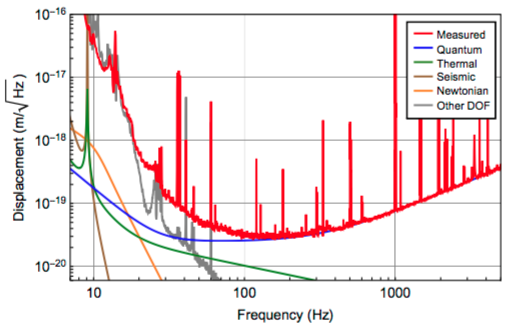
\includegraphics[width=.75\linewidth]{aligoNoise.png}
	\caption{This plot shows the theoretical noise sources, and the measured noise (red) in the interferometer.}
\end{figure}

\subsection{Noise Characteristics}
asdf

\subsection{Noise Elimination}
As mentioned before, most of the noise observed in data from LIGO is relatively Gaussian. By the same token, the proposed approach will assume the noise therein is Gaussian.

Let $\xi$ be the recorded signal. Assume we have a phase-modulated signal $X$ that has been adulterated with Gaussian noise $\epsilon$, which give rise to $\xi$:
\begin{equation}
\xi = X + \epsilon
\end{equation}

We first decompose the signal into intrinsic mode functions by empirical mode decomposition. 

\section{Possible Other Areas to Reasearch}
1) Instead of performing a Fourier Transform on the data f(t) maybe we could expand the data in terms of some other, cleverly chosen, set of orthogonal basis functions.  Is this viable and what would be the set of functions?  Can this reduce our search to a two dimentional search instead of a three dimentional search? (Task for Fourier Analysis Class MTH 490)

2) The LIGO interferometers sample the data at a finite frequency.  This introduces a maximum possible frequency of Gravitational Waves that can be detected, up to the Niquest Frequency.  This will, in tern, limit the maximum number of terms we can include in our sum (equation (9)).  What is the biggest $\omega_c$, $\Omega$, and $\Gamma$ that can be reasonably detected? (Task for Fourier Analysis Class MTH 490)

3) Obviously the duration of data is finite.  This puts a limit on how finly the Fourier Transform can resolve frequencies, ie. how small frequency bins can be.  This in tern tells us how small our step size in $\omega_c$ and $\Omega$ can be.  What are they? (Task for Fourier Analysis Class MTH 490)

4) Over very long periods of time $\omega_c \to 0$ because the neutron star loses energy/momentum to gravitational wave radation.  Over relatively much much shorter time periods $\Omega$ and $\Gamma$ change due to environmental reasons (not entirely sure on this).  What limitations does this put on our search, especially if the explicit nature of the time evolution of these parameters is unknown? ANSWER: it shortens the ammount of time we can take data over? (Task for Fourier Analysis Class MTH 490)

5) The Bessel Functions need to be calculated in a more efficient way.  What is it?  A basic investigation with Mathematica indicates we may only need to calculate the first $\Gamma$ terms or less.  That is if $\Gamma = 25.6830583$ then we may only need to take the sum in equation (10) to ~25 or so. (Task for Computational Physics Class PHY 480)

6) For any given value of $\Gamma$ there is a n such that $J_n(\Gamma)$ is maximized.  What is that n?  A basic investigation with a Mathematica script indicates $n \approx \Gamma$ is the answer.  How accurate is this approximation?  Can we show this analytically?  How many terms in equation (9) do we need to go out from n ~ $\Gamma$ do we need to go to get an accurate answer? (Task for Computational Physics Class PHY 480)

7) There are multiple data channels (because there are multiple observatories).  Could we compare data channels to help eliminate noise and pick out the exceptionally weak signals?

8) Some of the delta function type peaks on the noise spectrum (red) are known.  For example the 60Hz noise from power lines.  The LIGO scientists have ways of monitering this noise (they know the frequency, amplitude, and phase).  Does the data we obtain have this already subtracted off?  (Probably yes)  Curtis will look into this.

\section{Implementing the Gustafson Algorithm in C++ (Curtis Rau will do this for another class)}
Known problems with the algorithm include calculating large order bessel functions.  The bessel functions of natural number order are given by

\begin{equation}
J_n(z) = \sum_{m=0}^{\infty} \frac{(-1)^n}{m!(m+n)!} \left( \frac{z}{2} \right)^{2m+n}
\end{equation}

so calculating the nth Bessel function involves calculating factorials greater than n!.  The highest n for which we can store n! in an unsigned long integer type, the largest positive integer type, is 20:

\begin{align}
2^{64}-1 = 18,446,744,073,709,551,615 \\
< 21! = 51,090,942,171,709,440,000
\end{align}

if we are willing to sacrafise some precision to truncation we can use a double precision floating point integer which allows values upto $1.797,693,134,862,315,7 \cdot 10^{308}$

\begin{align}
170! \approx 7.25 \cdot 10^{306}				\\
< 1.797,693,134,862,315,7 \cdot 10^{308} < 	\\
171! \approx 1.24 \cdot 10^{309}
\end{align}

it has been shown that bessel functions up 250 or higher are necessary.  This whole buiseness of wresteling with factorials can be avoided by calculating the Bessel Functions using Bessel's Equation \ref{eqn:Bessel's Equation} \citep{folland}.

\begin{equation}
\label{eqn:Bessel's Equation}
x^2 J_n''(x) + x J_n'(x) + (x^2 + n^2) J_n(x) = 0
\end{equation}

To solve this second-order differential equation we will need two boundary conditions.  The boundary condition at $x=0$ is simple.

\begin{displaymath}
   J_n(x) = \left\{
     \begin{array}{lr}
       1 & : n = 0     \\
       0 & : n \neq 0
     \end{array}
   \right.
\end{displaymath}

For the other boundary condition we will use the asymtotic form of the Bessel functions.  Theorem 5.1 in \cite{folland} states:

\textit{For each $n \in N$ there is a constant $C_n \in R$ such that, if $x \geq 1$, then}

\begin{equation}
\left\| J_n(x) - \sqrt{\frac{2}{\pi x}} \cos \left( x - \frac{\pi}{4} (2n+1) \right) \right\| \leq \frac{C_n}{x^{3/2}}
\end{equation}

The standard perscription for numerically solving differential equations is first to discretize the independent variable $x \to x_i = x_{min} + i \cdot \delta x$.  Then use the limit definitions of the derivatives; we will use the three point definitions because their error goes as $O(\delta x^2)$ rather than using the two point definition with an error that goes as $O(\delta x)$.  Also, because there are only one order of Bessel Functions in Bessel's Equation, the order is implied by the $n$ that appears, so we will drop the subscript of $n$, $J_n \to J$, and we will further adopt the notation $J(x_i) = J_i$.

\begin{align}
J_i'  &= \frac{J_{i+1} - J_{i-1}}{2 \delta x} \\
J_i'' &= \frac{J_{i-1} - 2J_{i} + J_{i+1}}{\delta x^2}
\end{align}

So the discretized form of Bessel's Equation is

\begin{align}
\label{eqn:Bessel's Equation Discretized}
x_i^2 \frac{J_{i-1} - 2J_{i} + J_{i+1}}{\delta x^2} + x \frac{J_{i+1} - J_{i-1}}{2 \delta x} + (x^2 + n^2) J_i = 0
\end{align}

\begin{align}
\left(\frac{x_i^2}{\delta x^2} - \frac{x_i}{2\delta x}\right) J_{i-1}			\nonumber
	+ \left( \left(1-\frac{2}{\delta x^2}\right)x_i^2 - n^2 \right) J_i		\\
	+ \left(\frac{x_i^2}{\delta x^2} + \frac{x_i}{2\delta x}\right) J_{i+1}
	= 0
\end{align}

Where we have collected like terms of $J_i$.  For convenience we define coefficients to simplify the above equation.

\begin{align}
a_i &= \frac{x_i^2}{\delta x^2} - \frac{x_i}{2\delta x} 	\\
b_i &= \left(1-\frac{2}{\delta x^2}\right)x_i^2 - n^2  	\\
c_i &= \frac{x_i^2}{\delta x^2} + \frac{x_i}{2\delta x}
\end{align}



\appendix
\onecolumngrid
\section{The Fourier Transform of The Complex Function}
I BELIEVE I FORGOT SOME FACTORS OF 2PI HERE!!
Use the convolution theorem
Use the Jacobi-Anger expansion
Use the linearity of the Fourier Transform
Use the linearity of the Convolution
\begin{align}
F_t \left[ h_0 e^{i\left( \omega_0 t + \phi_0 + \Gamma \cos( \omega_1 t + \phi_1 ) \right)} \right]
&= h_0 e^{i\phi_0} F_t \left[ e^{i\omega_0 t} e^{i\Gamma \cos(\omega_1 t + \phi_1)} \right]													\\
&= h_0 e^{i\phi_0} F_t \left[ e^{i\omega_0 t} \right] \star \left[ e^{i\Gamma \cos(\omega_1 t + \phi_1)} \right]								\\
&= h_0 e^{i\phi_0} \delta(\omega - \omega_0) \star F_t \left[ \sum_{n=-\infty}^{\infty} i^n J_n(\Gamma) e^{in(\omega_1 t + \phi_1)} \right]		\\
&= h_0 e^{i\phi_0} \delta(\omega - \omega_0) \star \sum_{n=-\infty}^{\infty} i^n e^{in\phi_1} J_n(\Gamma) F_t \left[ e^{in\omega_1 t} \right]	\\
&= h_0 e^{i\phi_0} \delta(\omega - \omega_0) \star \sum_{n=-\infty}^{\infty} i^n e^{in\phi_1} J_n(\Gamma) \delta(\omega - n\omega_1)			\\
&= h_0 e^{i\phi_0} \sum_{n=-\infty}^{\infty} i^n e^{in\phi_1} J_n(\Gamma)  \delta(\omega - \omega_0) \star \delta(\omega - n\omega_1)			\\
&= h_0 e^{i\phi_0} \sum_{n=-\infty}^{\infty} i^n e^{in\phi_1} J_n(\Gamma)  \delta(\omega - \omega_0 - n\omega_1)
\end{align}


\begin{align}
F_t \left[ h_0 e^{i\left( \omega_0 t + \phi_0 + \Gamma \cos( \omega_1 t + \phi_1 ) \right)} \right] 			\nonumber
	&= \frac{h_0 e^{i\phi_0}}{\sqrt{2\pi}} \Huge{[} J_0(\Gamma) \delta(\omega - \omega_0) 					\\
	&+ \sum_{i=1}^{\infty} J_n(\Gamma) e^{-in\pi/2} 
	\left[ e^{in\phi_1} \delta(\omega - \omega_0 - n\omega_1) + e^{-in\phi_1} \delta(\omega - \omega_0 + n\omega_1) \right] \Huge{]}
\end{align}

\section{The Fourier Transform of The Real-Valued Function}

\begin{align}
F_t \left[ \Re \left\{ h_0 e^{i\left( \omega_0 t + \phi_0 + \Gamma \cos( \omega_1 t + \phi_1 ) \right)} \right\} \right]
&= \frac{1}{2} F_t \left[ h_0 e^{i\left( \omega_0 t + \phi_0 + \Gamma \cos( \omega_1 t + \phi_1 ) \right)} 
                        + h_0 e^{-i\left( \omega_0 t + \phi_0 + \Gamma \cos( \omega_1 t + \phi_1 ) \right)} \right]			\\
&= \frac{h_0}{2} \left[ 
  e^{ i\phi_0} F_t \left[ e^{i\left(  \omega_0 t + \Gamma \cos( \omega_1 t + \phi_1 ) \right)} \right] 
+ e^{-i\phi_0} F_t \left[ e^{i\left( -\omega_0 t - \Gamma \cos( \omega_1 t + \phi_1 ) \right)} \right] 
\right]
\end{align}

From the previous section we see that

\begin{align}
F_t \left[ e^{i(\omega_0 t + \Gamma \cos(\omega_1 t + \phi_1))} \right] 
= \sum_{n=-\infty}^{\infty} i^n e^{in\phi_1} J_n(\Gamma)  \delta(\omega - \omega_0 - n\omega_1)
\end{align}

and by replacing $\omega_0$ with $-\omega_0$ and $\Gamma$ with $-\Gamma$, and using the fact that $J_n(-\Gamma) = (-1)^n J_n (\Gamma)$ we also have

\begin{align}
F_t \left[ e^{i(-\omega_0 t - \Gamma \cos(\omega_1 t + \phi_1))} \right] 
= \sum_{n=-\infty}^{\infty} (-i)^n e^{in\phi_1} J_n(\Gamma)  \delta(\omega + \omega_0 - n\omega_1)
\end{align}

so the Fourier Transform of the real part of our frequency/phase modulated signal is

\begin{align}
F_t \left[ \Re \left\{ h_0 e^{i\left( \omega_0 t + \phi_0 + \Gamma \cos( \omega_1 t + \phi_1 ) \right)} \right\} \right]
&= \frac{1}{2} F_t \left[ h_0 e^{i\left( \omega_0 t + \phi_0 + \Gamma \cos( \omega_1 t + \phi_1 ) \right)} 
                        + h_0 e^{-i\left( \omega_0 t + \phi_0 + \Gamma \cos( \omega_1 t + \phi_1 ) \right)} \right]				\\
&= \frac{1}{2} h_0 e^{ i\phi_0} \sum_{n=-\infty}^{\infty} i^n e^{in\phi_1} J_n(\Gamma)  \delta(\omega - \omega_0 - n\omega_1)		\\
&+ \frac{1}{2} h_0 e^{-i\phi_0} \sum_{n=-\infty}^{\infty} (-i)^n e^{in\phi_1} J_n(\Gamma)  \delta(\omega + \omega_0 - n\omega_1)
\end{align}

\begin{align}
F_t \left[ \Re \left\{ h_0 e^{i\left( \omega_0 t + \phi_0 + \Gamma \cos( \omega_1 t + \phi_1 ) \right)} \right\} \right] 		\nonumber
&= \frac{h_0}{2\sqrt{2\pi}} \Huge{[} 
	  J_0(\Gamma) e^{ i\phi_0} \delta(\omega - \omega_0)	\color{red} + J_0(\Gamma) e^{-i\phi_0} \delta(\omega + \omega_0) 		\\
&+ \sum_{i=1}^{\infty} J_n(\Gamma) \Huge{[}																					\nonumber
     	X_n e^{ i\phi_0} e^{ in\phi_1} \delta(\omega - \omega_0 - n\omega_1) 
	  + X_n e^{ i\phi_0} e^{-in\phi_1} \delta(\omega - \omega_0 + n\omega_1)	\\
&+ \color{red}   Y_n e^{-i\phi_0} e^{-in\phi_1} \delta(\omega + \omega_0 + n\omega_1) 
   \color{red} + Y_n e^{-i\phi_0} e^{ in\phi_1} \delta(\omega + \omega_0 - n\omega_1)			
   \color{black} \Huge{]} \Huge{]}
\end{align}

Notice that, by taking the fourier transform of just the real part of our frequency modulated function it has added the terms in red.  (Go into more detail why that is)  The other important change is that the $X_n$ and $Y_n$ terms were added (Again, go into more detail why that is).  

% --------------------------- Code for the bibliography ---------------------------------------------------------------------------------
\twocolumngrid
\bibliography{shgBibliographyCopy}



\end{document}